\documentclass[12pt,English,a4paper,twoside,openright]{article}
\usepackage[utf8]{inputenc}
\usepackage[T1]{fontenc}
\usepackage[english]{babel}
\usepackage{graphicx}			%Figurer
\usepackage{fancyhdr}			%Fancy headere
\usepackage[pass]{geometry} 	%Sentrere Forside og tittelside
%\usepackage[european ports]{circuitikz} %Kretsdiagram
\usepackage{emptypage}
\usepackage[hidelinks]{hyperref}
\usepackage[hidelinks]{hyperref}
\usepackage{caption}
\usepackage[]{natbib} %referanser
\usepackage[section]{placeins}	%Holder floats innenfor seksjonen de er definert
\usepackage{blindtext} %Random fill
\usepackage{cleveref}
\usepackage{listings}
\usepackage{pdfpages}
\usepackage{url}
\usepackage{tikz-timing}
\usepackage{todonotes}
\lstset{basicstyle=\footnotesize\ttfamily,breaklines=true}

\newcommand{\blankpage}{
	\newpage
	\thispagestyle{empty}
	\mbox{}
	\newpage
}


			% Variables %
% % % % % % % % % % % % % % % % % % % % % % %
\newcommand{\MyAuthor}{Øystein Smith}
\newcommand{\MyTitle}{Portable and reliable DRSSTC demonstrator\\ }
\newcommand{\MyHeader}{\MyTitle}
\newcommand{\MyFag}{TFE4520 Prosjektoppgave}

% % % % % % % % % % % % % % % % % % % % % % % 

% Header og footer
\title{\MyTitle{}}
\author{\MyAuthor{}}
\fancyhead[C]{\MyHeader{}}
\fancyfoot[C]{\roman{page}}

\tolerance = 5000
\hbadness = \tolerance
\pretolerance = 2000

%%%%%%%%%%%%%%%%%%%%%%%%%%%%%%%%%%%%%%%%%%%%%%%%%%
\begin{document}

% %  Front page % %
% % % % % % % % %
\newgeometry{margin=2cm} %Sentrering av forside og tittelside
\begin{titlepage}
\thispagestyle{empty}
\centering
\textsc{\MyFag{}} \\[4cm]
\textsc{\LARGE Report} \\[1cm]
\textsc{\Huge \MyTitle{}}
\textsc{by} \\
\textsc{\MyAuthor{}} \\[2cm]
\textsc{\large \today}

%\maketitle
\begin{flushbottom}
\vfill

\includegraphics[scale=0.5]{img/ntnu} \\[0.5cm]
\textsc{\small FACULTY OF INFORMATION TECHNOLOGY, MATHEMATICS AND ELECTRICAL ENGINEERING \\ Norwegian University of Science and Technology}
\end{flushbottom}
\end{titlepage}

% Side 2 med kun tittel %
% % % % % % % % % % % % % % %
%Side 2 med kun tittel
\newpage
\thispagestyle{empty}
\textsc{}\\
[4cm]
\begin{center}
\textsc{\Huge \MyTitle{}}
\end{center}
\restoregeometry %Resten av dokumentet skal ikke være sentrert
\newpage

% Abstract %
%%%%%%%%%%%%%%%%%%%%%%%%%%%%%%%%%%%%%%%%%%%%%%%%%%
\pagestyle{fancy}
\setcounter{page}{1}
\label{abstract}
\begin{abstract}
Universities, knowledge centers and other institutions has the need for equipment that demonstrates physical phenomena in interesting and audience friendly ways. An example of this is a Double Resonant Solid State Tesla Coil (DRSSTC). It is desirable that the instrument is portable, reliable, and safe to use.

The system should take audio as input and output acoustic audio by means of an high voltage electric discharge in air creating plasma (streamer) by the means of a resonant transformer (tesla coil). The system should also be designed such that it will always be functional, and in the case of the system not being functional should fail in a safe and non-destructive way (safe having priority over non-destructive). As well as indicating witch part of the system is non-functional. The system should also be designed in such a way that this non-functioning part may be swapped for a spare functioning part. This was acheived with implementing a back plane architecture with detection of if modules are present, and signals that can be used by modules to report errors.

Before any improvements the system had a probability of failure P(F)= 0,71. After improvements we have removed F0 and F9 from the general fault tree, and F2, F3 from the destructive fault tree (F8) and the probability of failure is reduced to P(F)= 0,18. The probability for destructive failure P(F8) is reduced from 0,67 to 0,10.

The existing circuit design and implementation had problems with reliability. The reliability of the system was calculated by the use of a source tree based on logged faults to P(F)=0,71. After implementing a back plane design, and adding carrier wave detection on the input signal the reliability increased to P(F)=0,18. The probability of destructive failure was reduced from 0,67 to 0,10. This is a large increase in reliability. Portability was present in the existing implementation, and has been increased by removing failure sources that occurred when moving the system.


\end{abstract}
\newpage

% Preface (optional)% 
%%%%%%%%%%%%%%%%%%%%%%%%%%%%%%%%%%%%%%%%%%%%%%%%%%
\section{Preface}
\newpage

%Begin TOC
%%%%%%%%%%%%%%%%%%%%%%%%%%%%%%%%%%%%%%%%%%%%%%%%%%
\tableofcontents
\listoffigures
\listoftables
\cleardoublepage % begin on right page

% Begin DOC
%%%%%%%%%%%%%%%%%%%%%%%%%%%%%%%%%%%%%%%%%%%%%%%%%%
\pagestyle{fancy}
\fancyfoot[C]{\arabic{page}}
\setcounter{page}{1}

\section{Introduction}
\label{intro}
The system should take audio as input and output acoustic audio by means of an high voltage electric discharge in air creating plasma by the means of a resonant transformer (tesla coil). The system should also be designed such that it will always be functional, and in the case of the system not being functional should fail in a safe and non-destructive way (safe having priority over non-destructive). As well as indicating witch part of the system is non-functional. The system should also be designed in such a way that this non-functioning part may be swapped for a spare functioning part.

\subsection{Tesla}
\label{tesla}
The Tesla Coil or resonant transformer was invented by Nikolai Tesla and used for experiments with artificial illumination \citep{5570149}. Since then the Tesla Coil has become a popular entertainment device.
\todo{Write some words about Nikolai Tesla?}
\subsection{DRSSTC}
\label{DRSSTC}

\begin{figure}
    \centering
    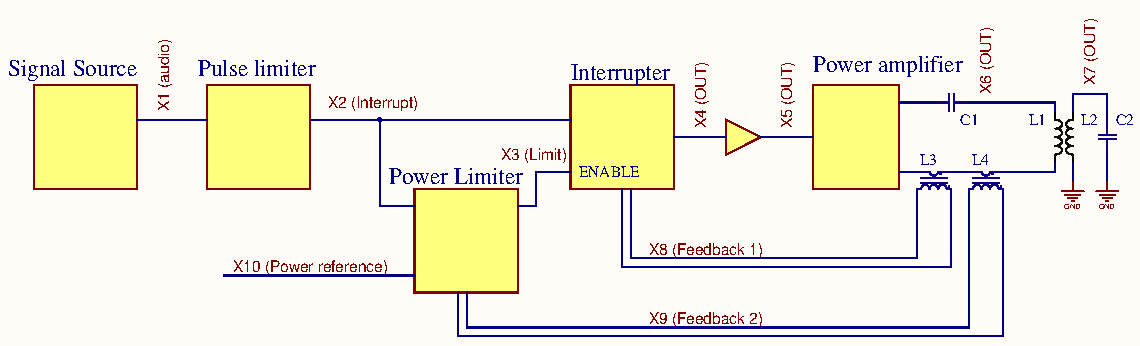
\includegraphics[width=\textwidth]{img/FunksjonsBlokkskjema.pdf}
    \caption{Block diagram}
    \label{fig:func_block}
\end{figure}

\begin{figure}
    \centering
    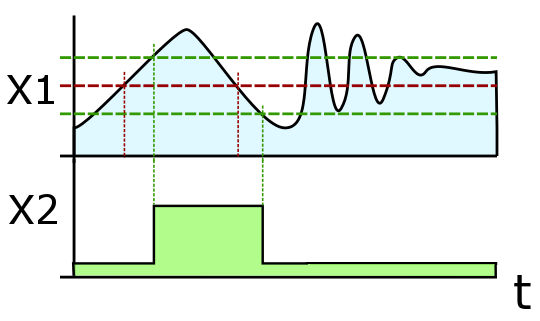
\includegraphics[width=\textwidth]{img/Smitt_hysteresis_graph_x1_x2.png}
    \caption{Tranformation of $X1$ to two level \citep{wikimedia}}       
    \label{fig:schmidt}
\end{figure}


DRSSTC is an acronym for Dual Resonant Solid State Tesla Coil. Dual resonant means that we have two resonant circuits inductively coupled, and tuned to the same resonance frequency. Solid state means that we drive these resonant circuits actively with transistors. The origins of the DRSSTC is not well documented but it is commonly accepted that it was conceived on "The tesla coil mailing list" \citep{pupman}.

The signal pathway consists of a signal source, pulse limiter, power limiter, interrupter, amplifier, and power amplifier see \cref{fig:func_block}.
The signal source provides the signal to be output on the coil, often the signal source is a musical recording.
The input signal should be monophonic, arpeggio\footnote{The sounding of the notes of a chord in rapid succession instead of simultaneously.} may be used. The input signal may be two level.

First the input signal $X1$ goes into the pulse shaper, which transforms the signal to two, level limits on-time of each pulse, and enforces a minimum time between pulses. In \cref{fig:schmidt} an example $X1$ is shown and a corresponding $X2$, here we see that the transformation to two level is done with a schmitd trigger, and that the pulses following immediately after the first pulse is suppressed. (\cref{timing_diagrams}). Then the signal X2 is connected to the interrupter which on a positive flank outputs a positive flank X4, which is amplified $X5$ and $X6$ and sent into the resonant circuit (C1, and L1). This triggers the step response of the resonant circuit. Then a positive feedback loop $X8$ drives $X4$ at the resonant frequency of the resonant circuit (the resonant frequency is in the order $f_0 = 100k$Hz). This is achieved by inverting the output when the current through C1 and L1 passes through zero (as measured through L3). This continues until either the input pulse $X2$ goes low or the limit signal from the limiter X3 goes low.
The limiter also measures the current flowing through C1 and L1, but this signal X9 is rectified and fed through a low pass filter before being compared to a preset level X10. This comparison measures the power dissipated in the resonant circuit. If the power exceeds the preset level the enable signal X3 is set low until the next rising edge of the input signal X2. X10 is set by a multi turn potentiometer.

The resonant circuitry consists of C1, L1, C2 and L2, where L2 is magnetically coupled with L1 with a degree of approximately 0.2. C1 is a bank of capacitors with high voltage and current rating and low equivalent series resistance (ESR). L1 is an inductor with high cross section area and few turns (in the magnitude of 5 turns). L2 is an inductor with low cross section area and a high number of turns (in the magnitude of 4000 turns). C2 consists of a sphere or toroid for one plate, and the grounded (safety ground) surroundings. Ground is connected through the safety ground in the electrical socket used to power the DRSSTC. L3 and L4 are current sensing transformers.

Figure \cref{fig:scope} shows a measurement of these signals. Channel 2 (Green) shows the feedback signal $X8$ after it is fed through a protection network limiting the voltage (See the schematic for TK514 in appendix B). Channel 4 (Red) shows an internal signal $Y1 = X2$ \&\& $\overline{X3}$ in the interrupter. This as long as this signal is high the output signal $X4$ will swing at the resonant frequency. Note that we would expect $X8$ to be zero as long as channel 4 is low, but there is some delay before the resonant circuit stops swinging after the supply of energy stops. Also note the interference on $X3$ and $Y1$ from the output signal $X6$.

\begin{figure}
    \centering
    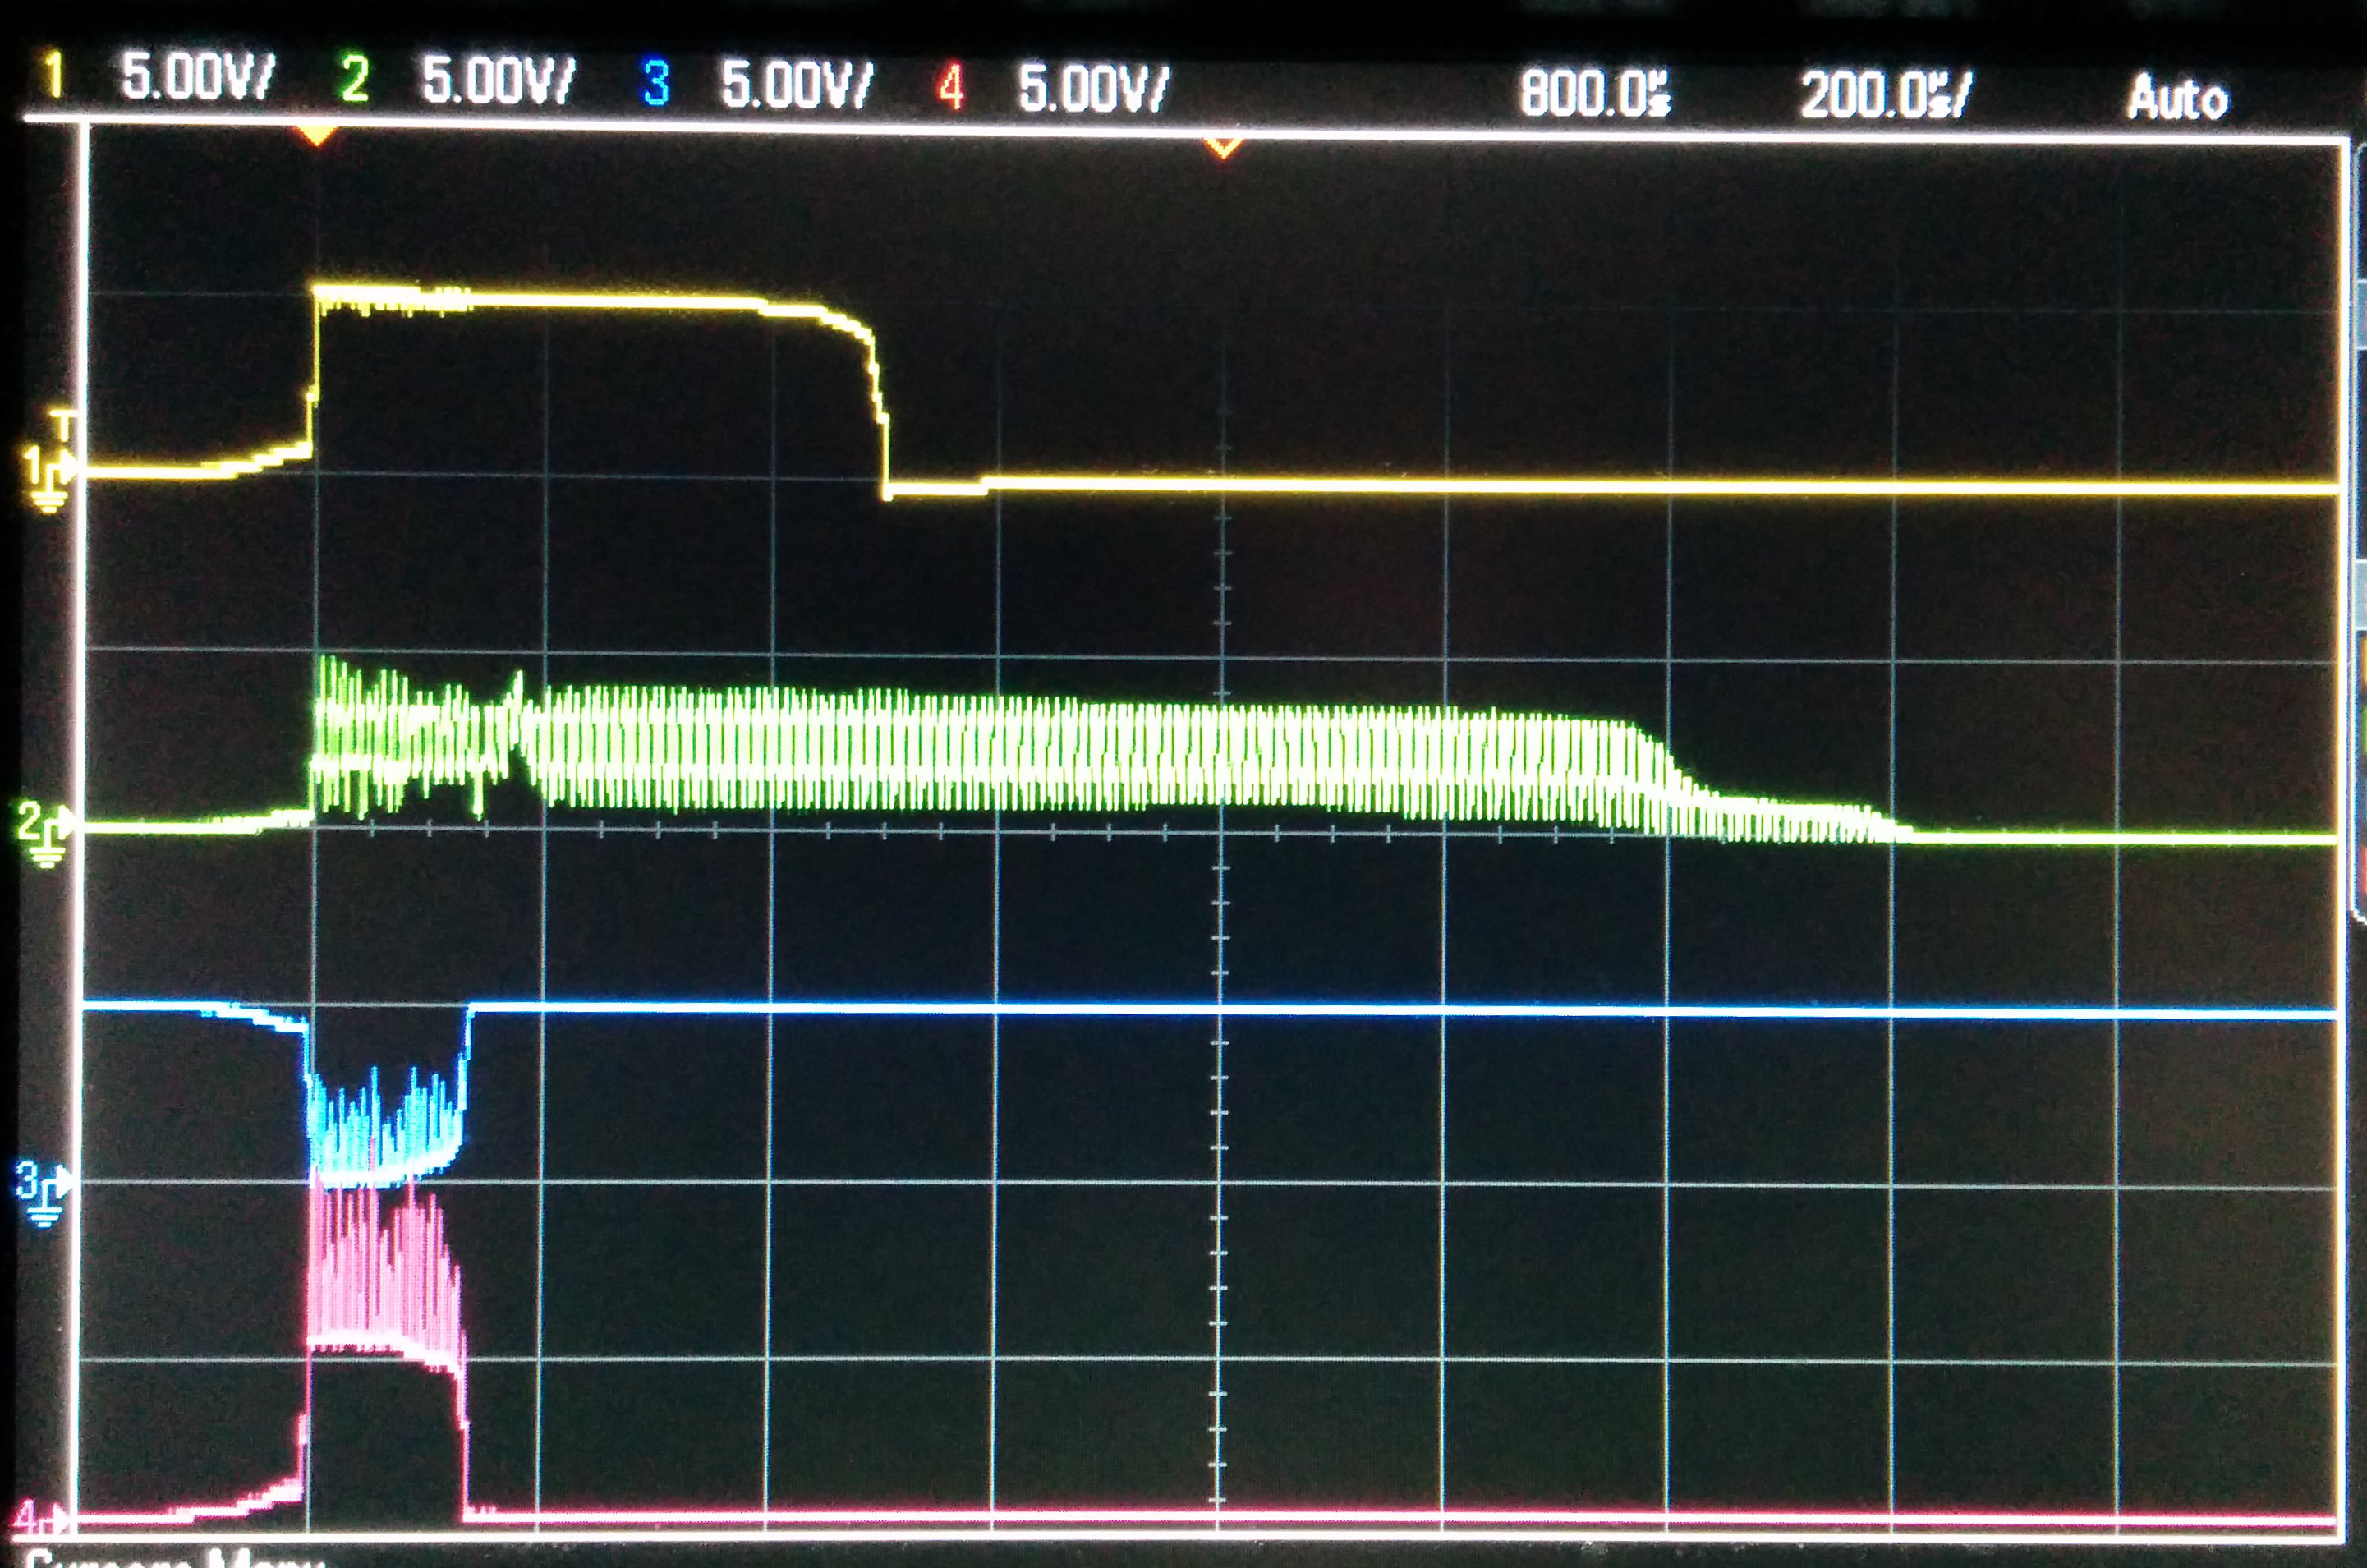
\includegraphics[width=\textwidth]{img/DRSSTC_scope.jpg}
    \caption{Measurements of signals.}
    \label{fig:scope}
    Channel 1 (Yellow): $X2$, 2 (Green): $X8$, 3 (Blue) $X3$, 4 (Red): $X2$ \&\& $\overline{X3}$. Voltage axis: 5V/div. Time axis: $200\mu$s/div.
\end{figure}

\subsubsection{Triggering signal}
\label{triggering_signal}
The triggering signal $X2$ is two level and contains two pieces of information from $X1$, the frequency $f$ (tone) and the volume (intensity). The frequency is given by the time $T$ between the positive flanks of the signal $f=\frac{1}{T}$. This is the base harmonic of the acoustic tone heard at the output of the system. The volume is given by the duty cycle of the pulses (the relationship between the pulse being high and the total period $T$ of the pulse. \Cref{fig:tones} shows different tones, and \cref{fig:volumes} shows different volumes.

\begin{figure}[!ht]
    \centering
    \begin{tikztimingtable}
        X2 & 2L 1H 7L 1H 7L 1H 7L 1H 7L\\
        X2 & 2L 1H 5L 1H 5L 1H 5L 1H 5L 1H 5L 1H 1L\\
    \end{tikztimingtable}
    \caption{Different tones}
    \label{fig:tones}
\end{figure}{}

\begin{figure}[!ht]
    \centering
    \begin{tikztimingtable}
        X2 & 2L 1H 7L 1H 7L 1H 7L 1H 7L\\
        X2 & 2L 3H 5L 3H 5L 3H 5L 3H 5L\\
    \end{tikztimingtable}
    \caption{Different volumes}
    \label{fig:volumes}
\end{figure}{}

\subsubsection{Timing diagrams}
\label{timing_diagrams}
\cref{fig:drsstc1} to \cref{fig:drsstc6} shows different examples of input pulses, and corresponding output pulses. Note that the timings and frequencies are not to scale, only relative timings.

\Cref{fig:drsstc1} shows a single pulse on the input signal $X1$, here we see $X2$ is limited to a certain width. We also see that $X4$ and $X8$ goes high when $X2$ goes high, oscillates at the resonance frequency of the resonance circuit, and goes low when $X2$ goes low. \Cref{fig:drsstc2} shows the same principle, only with a longer pulse on $X1$.

\Cref{fig:drsstc3} shows the same input signal as \cref{fig:drsstc2} but with a different setting of the on-time on the pulse limiter (allowing longer on-time).

\Cref{fig:drsstc4} to \cref{fig:drsstc6} shows multiple pulses on $X1$ and corresponding signals on $X2$. With on-time set to 2 units and minimum time between pulses set to 12 units.

\begin{figure}[!ht]
    \centering
    \begin{tikztimingtable}
        X1 & 5L 20H 18L\\
        X2 & 5L 10H 28L\\
        X3 & 43H \\
        X4 & 5L 10{1C} 28L\\
        X8 & 5L 10{1C} 28L\\
    \end{tikztimingtable}
    \caption{One pulse on X1}
    \label{fig:drsstc1}
\end{figure}{}

\begin{figure}[!ht]
    \centering
    \begin{tikztimingtable}
        X1 & 5L 30H 8L\\
        X2 & 5L 10H 28L\\
        X3 & 43H \\
        X4 & 5L 10{1C} 28L\\
        X8 & 5L 10{1C} 28L\\
    \end{tikztimingtable}
    \caption{One pulse on X1, longer input pulse}
    \label{fig:drsstc2}
\end{figure}{}

\begin{figure}[!ht]
    \centering
    \begin{tikztimingtable}
        X1 & 5L 30H 8L\\
        X2 & 5L 20H 18L\\
        X3 & 20H 23L\\
        X4 & 5L 15{1C} 23L\\
        X8 & 5L 15{1C} 23L\\
    \end{tikztimingtable}
    \caption{One pulse on X1, longer on time}
    \label{fig:drsstc3}
\end{figure}{}

\begin{figure}[!ht]
    \centering
    \begin{tikztimingtable}
        X1 & 5L 10H 10L 10H 8L\\
        X2 & 5L 2H 18L 2H 16L\\
    \end{tikztimingtable}
    \caption{Multiple pulses on X1 (max on: 2, min between: 12)}
    \label{fig:drsstc4}
\end{figure}{}

\begin{figure}[!ht]
    \centering
    \begin{tikztimingtable}
        X1 & 5L 10{4C}\\
        X2 & 5L 2H 14L 2H 14L 2H 6L\\
    \end{tikztimingtable}
    \caption{Multiple pulses on X1 (max on: 2, min between: 12)}
    \label{fig:drsstc5}
\end{figure}{}

\begin{figure}[!ht]
    \centering
    \begin{tikztimingtable}
        X1 & 5L 8{5C}\\
        X2 & 5L 2H 18L 2H 18L\\
    \end{tikztimingtable}
    \caption{Multiple pulses on X1 (max on: 2, min between: 12)}
    \label{fig:drsstc6}
\end{figure}{}
\subsubsection{Model of DRSSTC}
\subsection{Reliability}
\label{reliability}
In every system there is certain demands for reliability (reliablilty describes the ability of a system to function under certain condiditons for a specified period of time). The DRSSTC should function in indoor conditions and dry outdoors weather, the DRSSTC should also function after sitting in storage for up to one year. And should function after transportation by trolley and or car. And after sitting on a stage during rigging. The DRSSTC should function for several years with transportation and rigging up to 30 times a year.

To achieve this the system should also have high maintainability. It should take a maximum of one day to fix an error.

\subsubsection{Fault tree}
A method for analyzing reliability of a system is using a fault tree \citep{faulttree}. The fault trees for this system is shown in \cref{fig:ftree_drsstc_dest} and \cref{fig:ftree_drsstc}. The inputs are failure sources that can occur these are listed in \cref{tab:fail_sources}. The probability P for each failure source is calculated from the number of times this failure has occurred divided by the number times the system has been used. These numbers are extracted from the log entries in Omega Verksteds log book for their tesla coil \citep{teslalog}. A total of 33 uses are logged in the period 2013-08-22 to 2016-11-07, the real number of uses should be assumed higher as the log book is not written at each use due to human error. The fault sources that does not occur in the log book is assumed to have a probability P of less than 0,03. Some of these failure sources are due to operator error and is outside of this report to fix. These failures sources are F3, F5, and F7 they are attempted to fix with procedures \citep{teslaprosedyrer}. The failure source with the highest probability $P=0,12$ is F8 this is a failure that does not occur by itself but as a consequence of other failure sources as shown in \cref{fig:ftree_drsstc_dest} and must thus be fixed by addressing the failure sources leading to this failure. The failure source remaining with the highest probability $P=0,09$ is F2 defective optical cable. By using the standard rules of combining probabilities with logic functions we get a calculated probabiliy of failure of P(F)= 0,71. The probability for destructive failure P(F8) used in calculating the probability for failure P(F) is the value gotten from calculating the output from the destructive failure fault tree P(F8)=0,666, and not the value listed in \cref{tab:fail_sources}.

\begin{table}[h]
    \centering
    \begin{tabular}{|p{0.05\textwidth}|p{0.1\textwidth}|p{0.75\textwidth}|}
        \hline
        & P & Description \\ \hline
        F0 & 0,03 & System is transported and vibrations shakes loose the wires on the high voltage side of the system.  \\ \hline
        F1 & <0,03 & No carrier wave (CW) detection is implemented in the optical reciever of the driver TK500, or this detection is defective.\\ \hline
        F2  & 0,09 & Optical cable is defective (someone has stepped on it).\\ \hline
        F3  & 0,03 & Optical cable is missing.\\ \hline
        F4  & < 0,03 & Pulse shaper (TK100) is defective.\\ \hline
        F5  & 0,06 & Pulse shaper is set to too high volume.\\ \hline
        F6  & 0,03 & Power limiter is defective.\\ \hline
        F7  & 0,06 & Power limiter is set to too high power.\\ \hline
        F8  & 0,12 & Destructive failure happens, power amplifier or the load capacitor C1 catches fire. \\ \hline
        F9  & 0,03 & Internal cables are disconnected due to vibrations while transporting the system. \\ \hline
    \end{tabular}
    \caption{Failure sources}
    \label{tab:fail_sources}
\end{table}

\begin{figure}[h]
\begin{circuitikz}[scale = 0.65, transform shape] \draw
(0,0) node[] (x0){F7: Limiter settings}
(0,1.2) node[] (x1){F6: Limiter def.}
(0,2) node[] (x2){F5: Sig. gen settings}
(0,2.8) node[] (x3){F4: Sig. gen def.}
(0,4) node[] (x4){F3: Optical cable missing}
(0,5) node[] (x5){F2: Optical cable def.}
(0,6) node[] (x6){F1: CW detection def.}
(0,7) node[] (x7){F0: HV cables disconnected}
(15,2) node[] (x8){F8: Destructive failure}
(4,6.5) node[or port] (myor1) {}
(4,4.5) node[or port] (myor2) {}
(4,2.5) node[or port] (myor3) {}
(6,1.5) node[and port] (myand1) {}
(8,2.5) node[or port] (myor4) {}
(10,3) node[and port] (myand2) {}
(12,2) node[or port] (myor5) {}
(x0) -- (10,0) -- (myor5.in 2)
(x1) -- (myand1.in 2)
(x2) -- (myor3.in 2)
(x3) -- (myor3.in 1)
(x4) -- (myor2.in 2)
(x5) -- (myor2.in 1)
(x6) -- (myor1.in 2)
(x7) -- (myor1.in 1)
(myor5.out) -- (x8)
(myor1.out) -- (myand2.in 1)
(myor2.out) -- (myor4.in 1)
(myor3.out) -- (myand1.in 1)
(myand1.out) -- (myor4.in 2)
(myor4.out) -- (myand2.in 2)
(myand2.out) -- (myor5.in 1);
\end{circuitikz}
\caption{Fault tree for destructive failure of DRSSTC}
    \label{fig:ftree_drsstc_dest}
\end{figure}

\begin{figure}[h]
\begin{circuitikz} \draw
(0,2) node[] (x0){F8: Destructive failure}
(0,1) node[] (x1){F9: Internal cables missing}
(0,0) node[] (x2){F2: Optical cable defective}
(8,1.5) node[] (x3){Failure}
(4,0.5) node[or port] (myor1) {}
(6,1.5) node[or port] (myor2) {}
(x0) -- (myor2.in 1)
(x1) -- (myor1.in 1)
(x2) -- (myor1.in 2)
(myor1.out) -- (myor2.in 2)
(myor2.out) -- (x3);
\end{circuitikz}
\caption{Fault tree for non-destructive failure of DRSSTC}
    \label{fig:ftree_drsstc}
\end{figure}

% Fault tree diagram

% Utgangstrinn blåser = For mye effekt = (limiter feil innstilt || limiter defekt ) && ( (Signalgenerator feil innstilt || sig. gen defekt) || (optisk kabel detti ut && bærebølgedeteksjon def.) )
% ledninger mellom moduler detter ut
% Mosfetdrivere blåser = ?
% utgangskondensator blåser = For lav rating på kondis ? for høy effekt
% optisk inn dør = tråkket på
% overslag mellom ting på hv siden etter risting
% utgangskabelen smelter

\subsubsection{Maintainability}
The goal of errors taking a maximum of one day to fix is set so that you will always have a functioning system by testing it one day before it is to be used for a performance. By partitioning the system into modules with limited components, the assembly time for one module is kept short. By keeping spare modules, and spare components. You will be able to either just switch the module, wich by the use of a backplane takes only a matter of minutes. Or assemble a new module wich should take less than one day.
\subsection{Mass producability}

\subsection{Customer}
The customers of the system is Omega Verksted, research projects, and amusement parks. These customers can be divided into two groups, customers who will be moving the DRSSTC and packing it down when not in use, and customers who will have it in a permanent installation. We will focus on the customers moving the DRSSTC around since this will put the toughest requirements on the design.
\section{System Architecture}
\subsection{Card inserted bus}

\section{Specification}
The overall specification of the system is described in \cref{intro}.

One of the dangers with a DRSSTC is injury or death by electrocution, the safest and most practical way to prevent this is by a set of procedures regarding operation\todo{Reference procedures}, and the possibility to disconnect the coil rig from the rest of the system easily. To be able to disconnect the coil rig easily a user friendly connector should be used.

A failure mode is the coil rig catching fire due to too much power dissapation, the power limiter should prevent this. Bærebølgedeteksjon, plugging av signalkabel.
\todo{Spesifisere hva som skal være trygt, hvordan kan det være farlig?}

By non-destructive failure propagation we mean that the failure of one module should not propagate to another module. Or lead to the coil rig catching fire or outputting high voltage when it is not expected.
\todo{Spesifisere non-destructive failure propagation}

\todo{Overvåkningsfunksjonalitet i systemet}

\todo{Funkjsonelle krav, ikke funksjonelle krav.}



With this specification in mind the system has been partitioned into sub-systems listed below. The sub systems has been assigned an arbitrary part number with the prefix "TK".

\begin{figure}
    \centering
    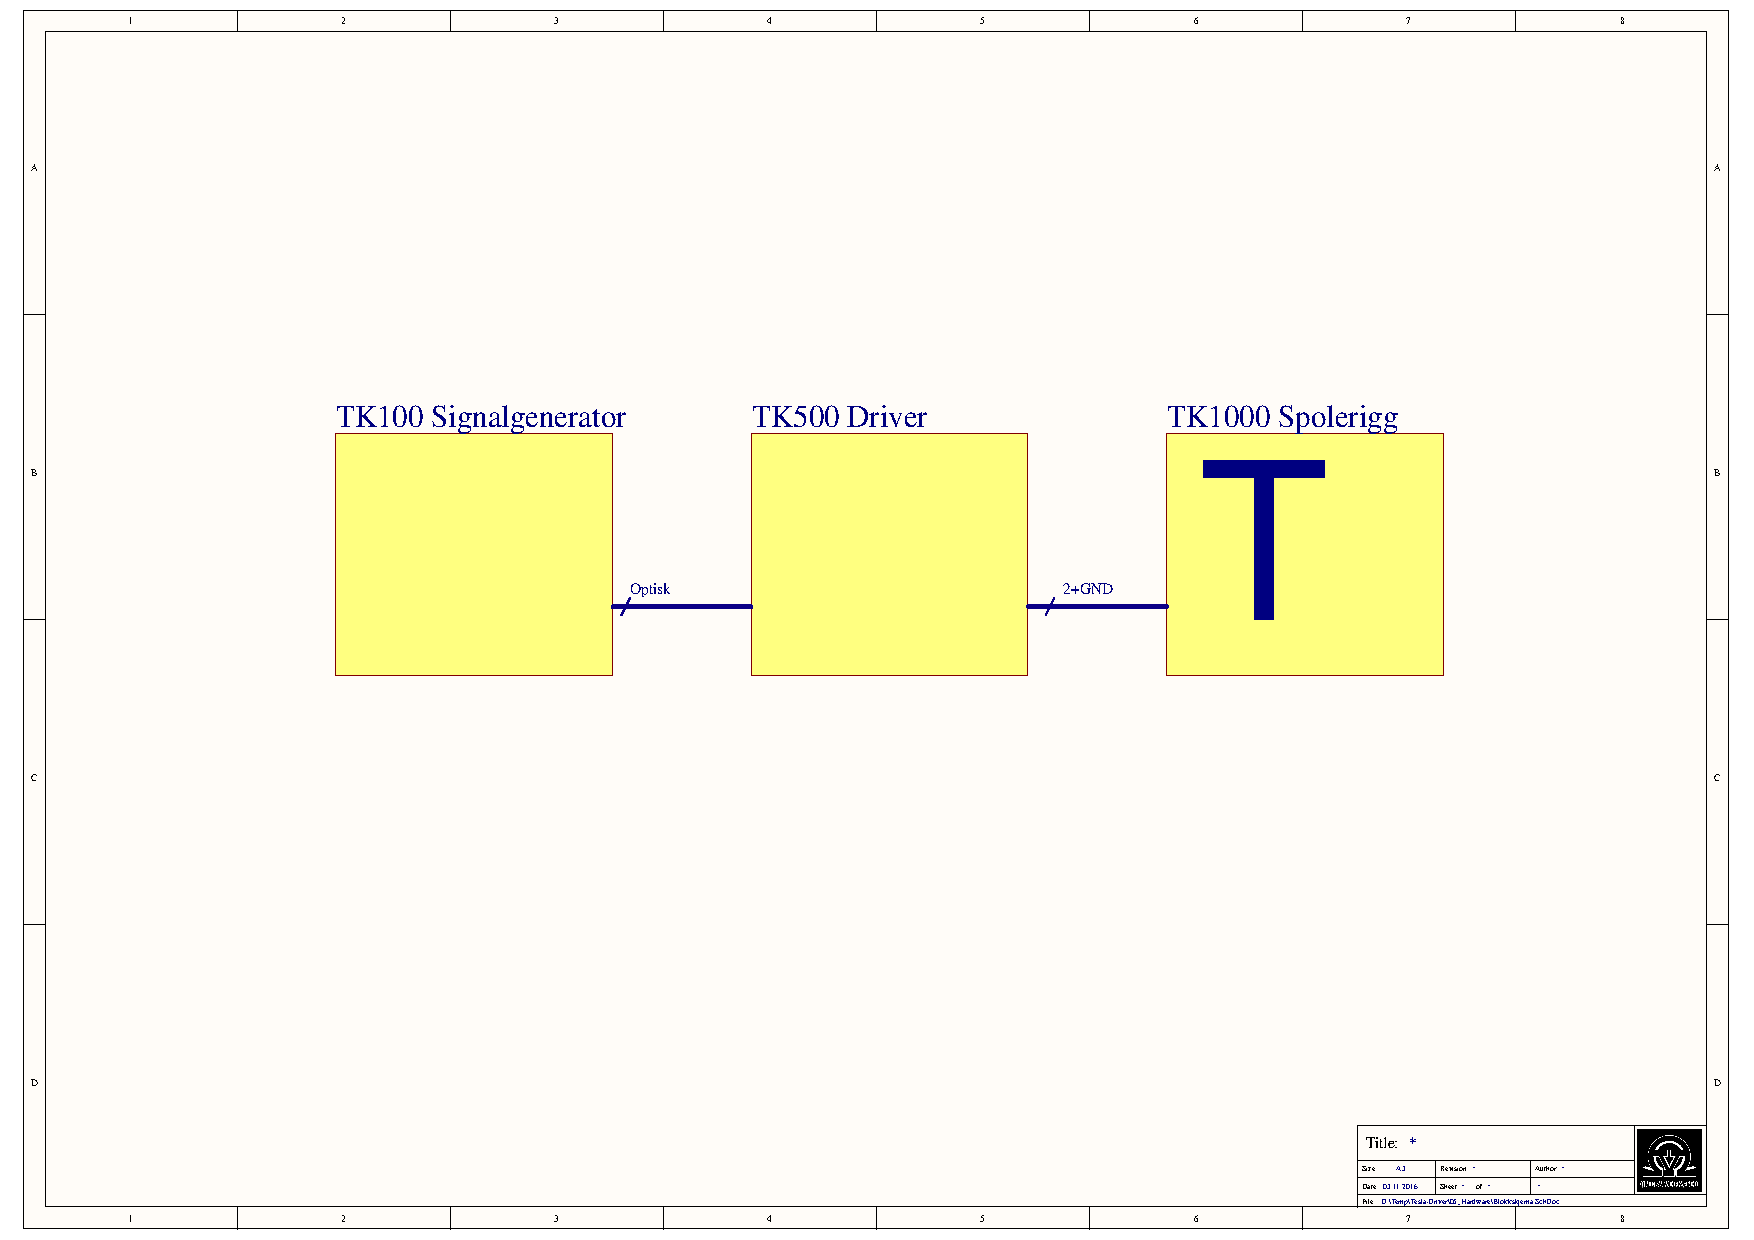
\includegraphics[trim={5cm 9cm 4.8cm 6.5cm},clip,width=\textwidth]{img/Blokkskjema.pdf}
    \caption{Block diagram}
    \label{fig:blokksjema}
\end{figure}

\begin{figure}
    \centering
    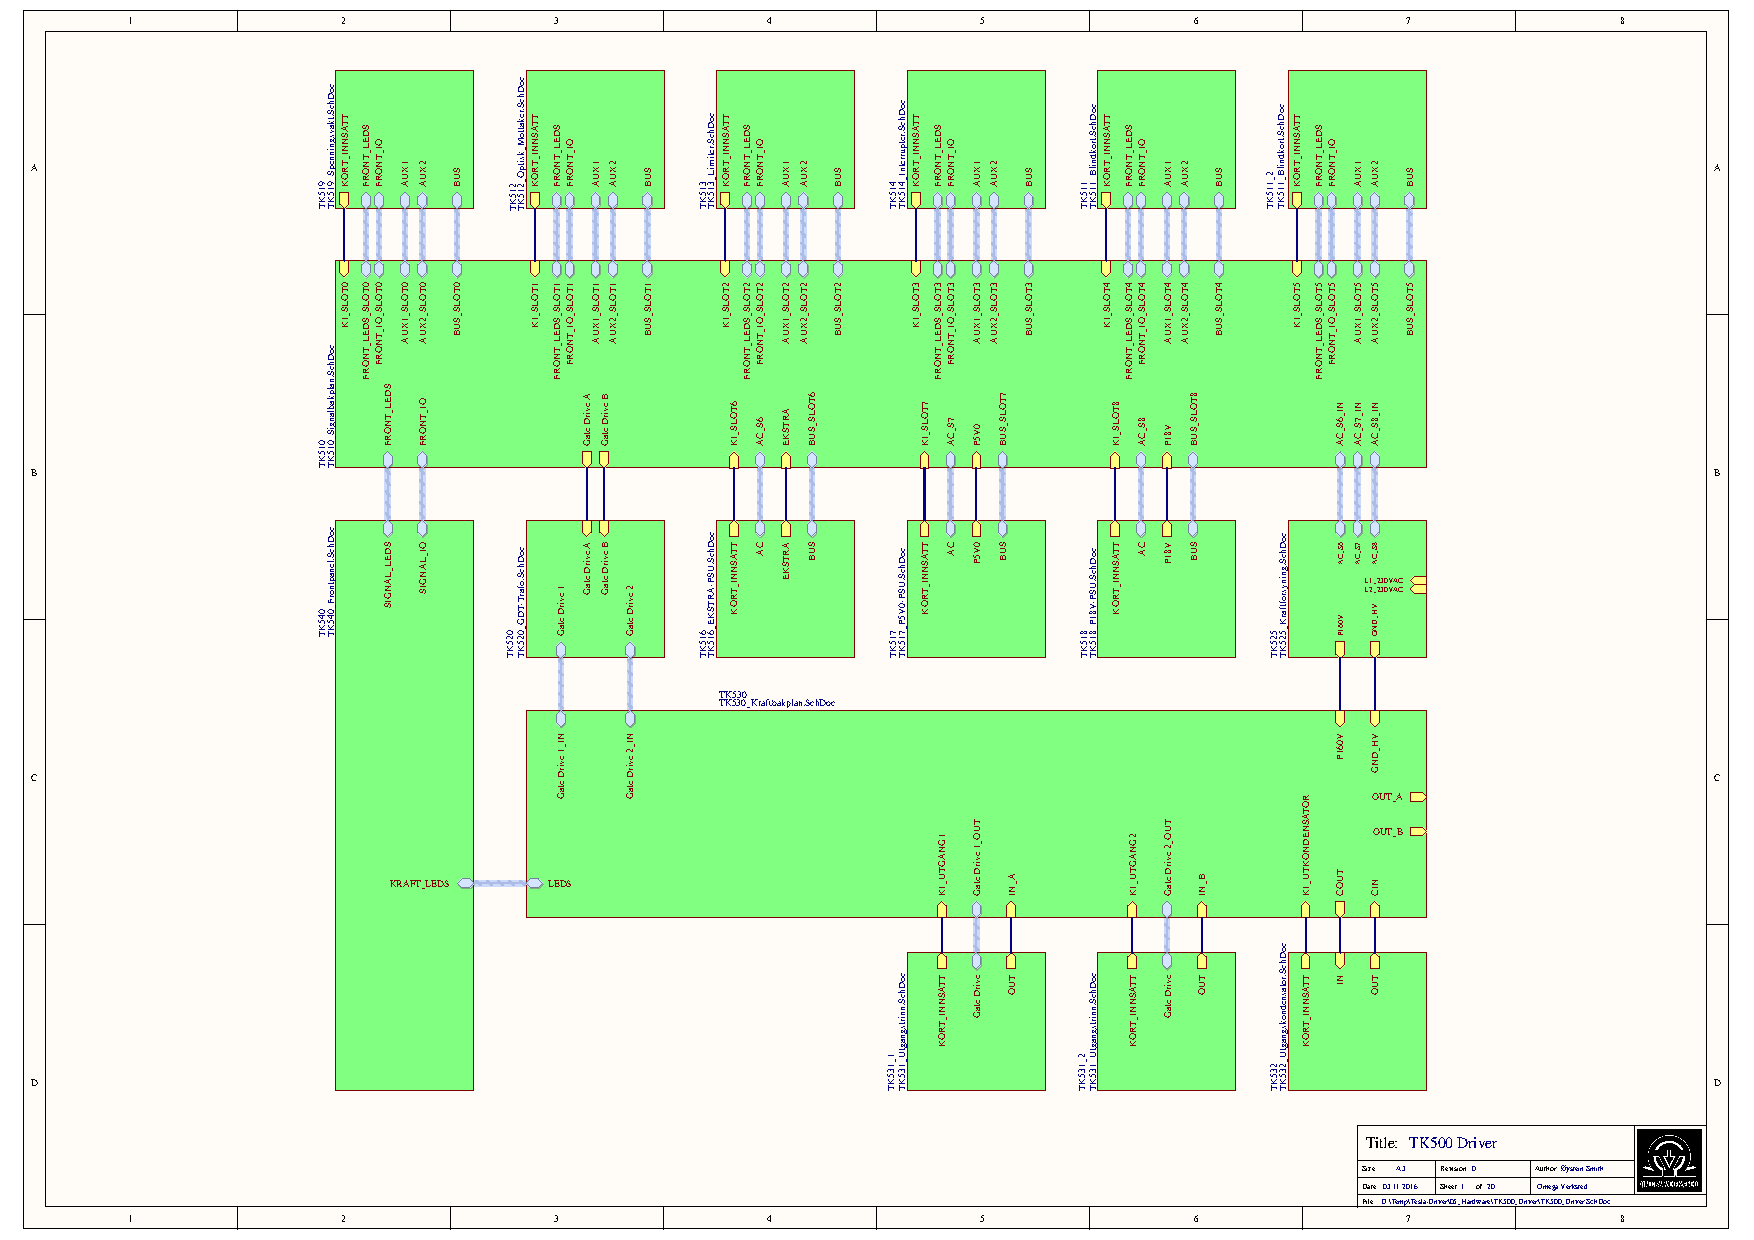
\includegraphics[trim={5cm 2cm 5cm 1cm},clip,width=\textwidth]{img/TK500_Driver.pdf}
    \caption{Block diagram of TK500 Driver}
    \label{fig:tk500}
\end{figure}

\begin{enumerate}
    \item TK100 Signalgenerator
    \item TK500 Driver
    \begin{enumerate}
        \item TK501 Frontpanel
        \item TK502 Frontpanel LEDS
        \item TK510 Signalbakplan
        \item TK511 Blindkort
        \item TK512 Optisk Mottaker
        \item TK513 Limiter
        \item TK514 Interrupter
        \item TK516 Ekstra-PSU
        \item TK517 P5V0-PSU
        \item TK518 P18V-PSU
        \item TK519 Spenningsvakt
        \item TK520 GDT-Trafo
        \item TK530 Kraftbakplan
        \item TK531 Utgangstrinn
        \item TK532 Kondensatorkort
    \end{enumerate}
    \item TK1000 Spolerigg
\end{enumerate}

\subsection{TK100 Signal generator}
The Signal generator Should take a wide range of inputs and output the triggering signal X2 for the driver. It consists of the pulse shaper and signal source mentioned in \cref{DRSSTC} and shown in \cref{fig:func_block}. The output signal X2 should be sent through a optical plastic fibre to be against EMI as mentioned in \cref{sa} and \cref{optical}. The output signal should also be modulated on a carrier wave as described closer in \cref{triggering_signal} and \cref{carrier_wave}.
\todo{Navn på signaler her og i arkitekturseksjonen må stemme med hverandre}

\subsubsection{Triggering signal}
\label{triggering_signal}
The triggering signal X2 should be in the hearable frequency range with a configurable maximal pulse width (high) in the approximate range $0\mu$s - $800\mu$s. The triggering signal should also have a configurable minimum time between pulses.
\subsubsection{Carrier wave}
\label{carrier_wave}
The carrier wave CW for the optical channel should have a sufficiently high frequency $f=\frac{1}{T}$ to transfer the triggering signal X2, in addition to be easily detected in the receivinvg end.\todo{Reference figure in section about optical channel} X2 contains two parts of information the positive flank determining when the tesla coil fires. and the duration of the positive pulse determining the power output (volume). The period $T$ should be shorter than the lowest desirable positive pulse on X2 $T_{X2min}$. \todo{Double check value from experiment} $f_{CW} > \frac{1}{T_{X2min}}$
The shortest desirable pulse on X2 is a length that allows turning the volume down without a noticeable step before shutoff.

\subsubsection{Modulation}
\label{modulation}
The triggering signal should be pulse width modulated PWM with a logical high having a duty cycle of 80\% and logical low having a duty cycle of 20\%.
\begin{figure}[h!]
    \centering
    \begin{tikztimingtable}
        CW (2MHz) & L 17{2C} G 1L \\
        Triggering Signal $X2$ & 9L 8H 19L \\
        PWM & 1L 1H 3L 1H 3L 3H 1L 3H 1L 1H 3L 1H 3L 1L 1H 3L 1H 3L 1L 1H \\
    \end{tikztimingtable}
    \caption{Modulated signal timing diagram}
    \label{fig:cs_td}
\end{figure}{}

\subsection{TK500 Driver}

The driver should take the output of the signal generator (TK100) as input, and output a 160VDC signal at the resonant frequency of the coil rig while the input signal is high and the peak power output does not exceed a configurable level. The driver should also have the capacitor of the primary resonant circuit integrated.

\subsubsection{TK501 Frontpanel}
Should have a height of 4 standard rack units (4U) (17.78cm). Partitioned into multiple parts.
\subsubsection*{Signal back plane card matrix}
Use the entire height, height divided into equal parts for each card in the signal back plane card. Each division should contain four LEDs; Green (Card inserted), Red (Fault), Green (status), Yellow (led in button). A field for card name. Space for buttons depending on the needs of the specific card.

\subsubsection*{Power back plane card matrix}
Three leds for each of the three cards in the power back plane. Green (card inserted), Red (fault), Green (status).

\subsubsection*{Display}
Voltage meter for output voltage.
Ampere meter for output current.

\subsubsection*{Power buttons}
Emergency stop
Spring loaded rotary switch: slow start
Momentary switch: Power on
Momentary switch: Power off

\subsection{TK510 Signalbakplan}
The signal back plane should have six slots for signal modules, and three slots for power supplies.

\subsubsection{Signal module slot}
The signal module slot should have the following signals:
\begin{itemize}
    \item 1 bus with straps for pull up and pull down on bus lines. (B1-B14)
    \item Card inserted detection (A1)
    \item LED signals to front panel (A1-A5)
    \item Misc signals to front panel (A6-A10)
    \item Two contacts for signals other places inside chassis (A11-A14)
    \item Supply voltages and ground (A15-A18 \& B15-B18)
\end{itemize}
The pinout on the module slot connector is shown in \cref{fig:signalmodulslot}

\begin{figure}[h]
    \centering
    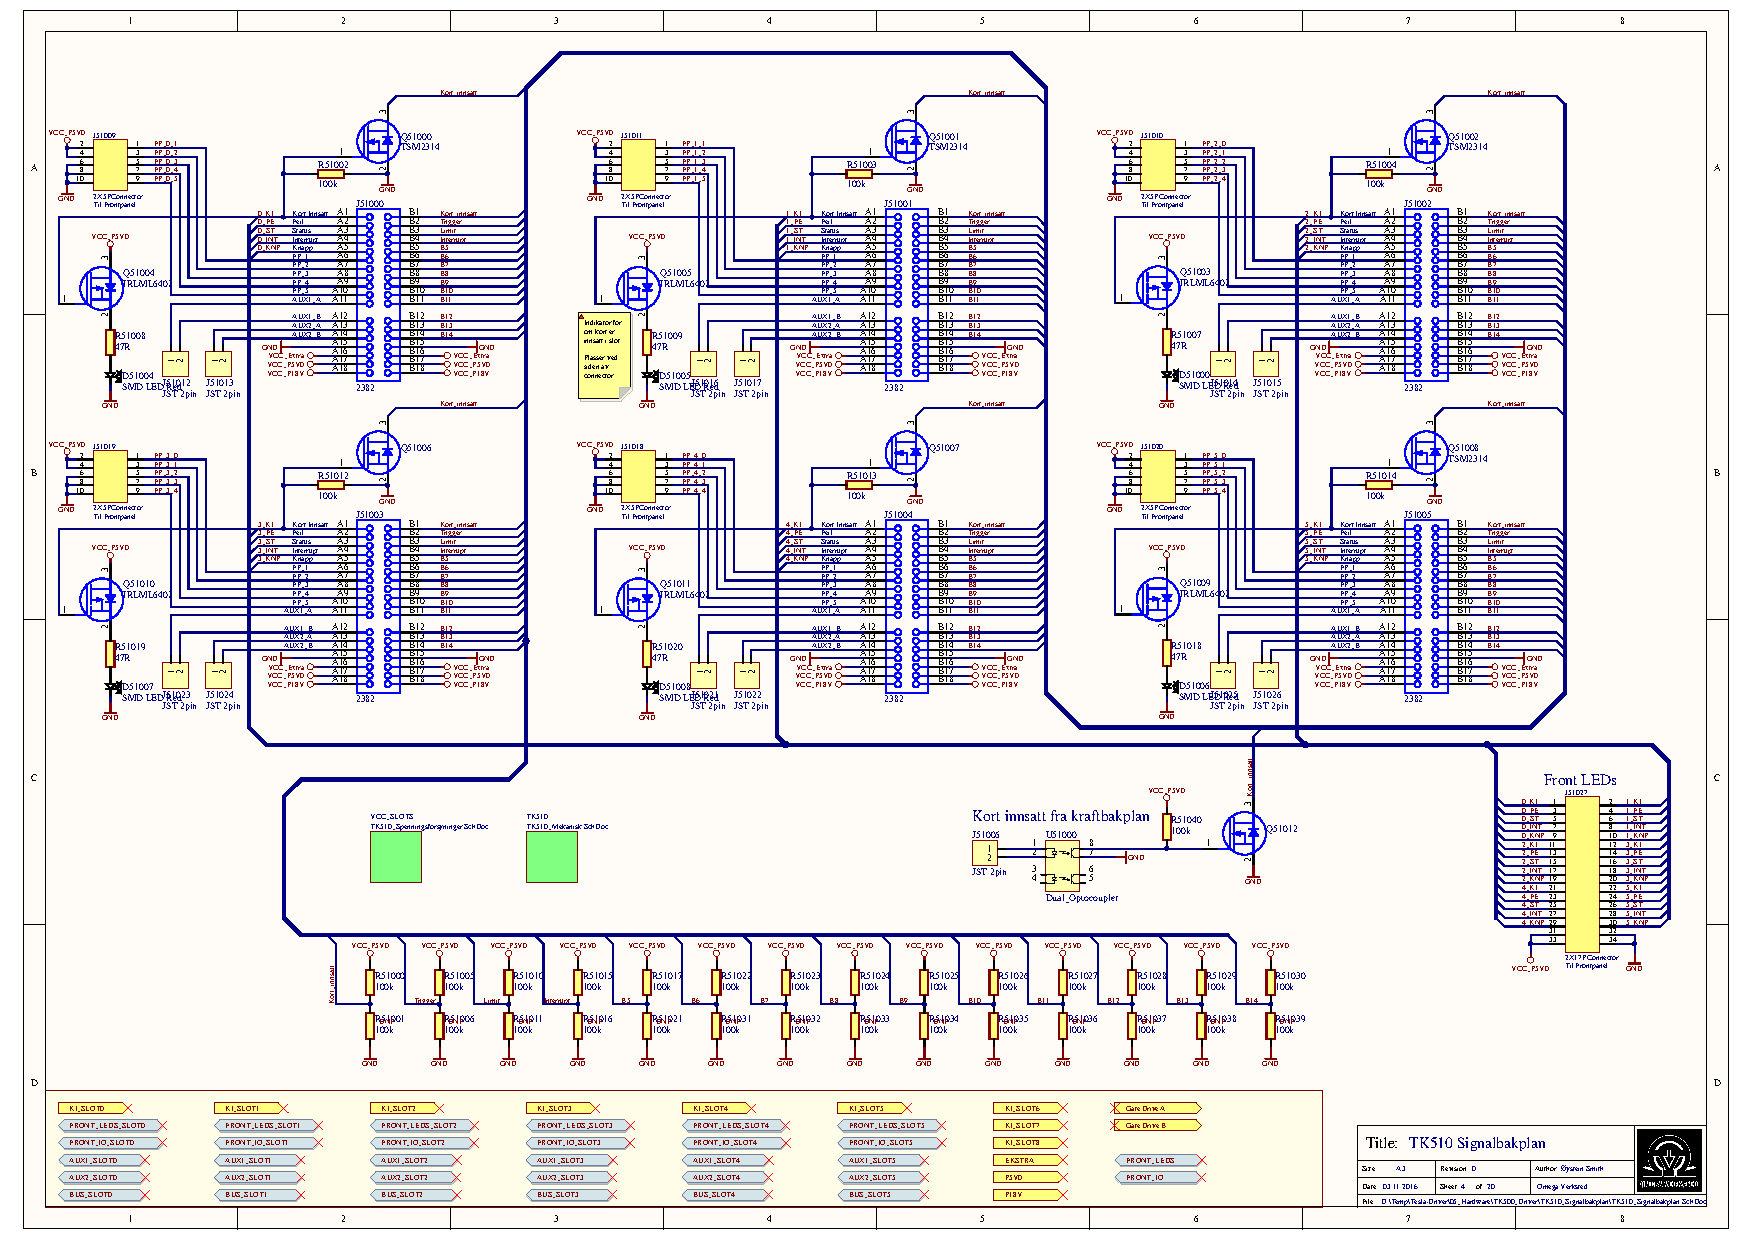
\includegraphics[trim={4.1cm 14.3cm 21.2cm 3.3cm},clip,width=\textwidth]{img/TK510_Signalbakplan.pdf}
    \caption{Signal module card slot connector (detail from schematic of TK510 Signalbakplan)}
    \label{fig:signalmodulslot}
\end{figure}

\subsection{TK511 Blindkort}
The purpose of $TK511$ is to take the space where no module is inserted into the signal back plane, and emulate an inserted module.

\subsection{TK512 Optisk Mottaker}
The purpose of $TK512$ is to convert the optical signal input into the driver $TK500$ to an electrical signal, and a carrier wave detected signal.

\subsection{TK513 Limiter}
The purpose of $TK513$ is to prevent the coil rig $TK1000$ from catching fire, and to keep the spark from turning yellow.

\subsection{TK514 Interrupter}
The purpose of $514$ is to fire the tesla coil when receiving input signal and to tune the output signal via a positive feedback loop to the systems resonance frequency.

\subsection{TK516 Ekstra-PSU}
The purpose of $TK516$ is to reserve a slot for future voltages.

\subsection{TK517 P5V0-PSU}
The purpose of $TK516$ is to provide 5V DC to the driver $TK500$.

\subsection{TK518 P18V-PSU}
The purpose of $TK516$ is to provide 18V DC to the driver $TK500$.

\subsection{TK519 Spenningsvakt}
The purpose of $TK516$ is to monitor the supply voltages in the driver $TK500$.

\subsection{TK520 GDT-Trafo}
The purpose of $TK516$ is to provide galvanic isolation between the signal back plane and the power back plane.

\subsection{TK530 Kraftbakplan}
The purpose of $TK516$ is to provide the connections and monitoring for the output stage $TK531$ and the load capacitor $TK532$.

\subsection{TK531 Utgangstrinn}
The purpose of $TK516$ is to step up the voltage on the output.

\subsection{TK532 Kondensatorkort}
The purpose of $TK516$ is to provide the capacitance of the primary resonance circuit.

\subsection{TK1000 Spolerigg}
The purpose of $TK516$ is to look good and output the voltage arc or corona discharge.
\section{Increasing Reliability}
\subsection{Sub module detection}
\subsection{Communication between modules}
\subsection{Bus}
\section{User interface}
\section{Schematics}
\section{Layout}
\section{Assembly}
\section{Testing}
\subsection{Measurements(techniques)}
\subsection{Results}
\section{Discussion}
\section{Conclusion}

% Referanser (biblatex) %
% % % % % % % % % % % % % % % % % % % % % %
\newpage
\bibliographystyle{plain}
\bibliography{ref}
\end{document}
